\documentclass[prodmode,acmtecs]{acmsmall} % Aptara syntax

\usepackage{amssymb}
\usepackage{amsmath}
\usepackage[margin=1in]{geometry}
\usepackage{exscale}
\usepackage[]{graphicx}
\usepackage[]{graphics}
\usepackage{listings}
\usepackage{float}

% Package to generate and customize Algorithm as per ACM style
\usepackage[ruled]{algorithm2e}
\renewcommand{\algorithmcfname}{ALGORITHM}
\SetAlFnt{\small}
\SetAlCapFnt{\small}
\SetAlCapNameFnt{\small}
\SetAlCapHSkip{0pt}
\IncMargin{-\parindent}

% no indentation - just spaces between paragraphs
\usepackage[parfill]{parskip}

%%%%%%%%%%%%%%%%%%%%%%%%%%%%%%%%%
\setcounter{tocdepth}{2}

\newcommand{\qt}[1]{``#1''}
\newcommand{\code}[1]{\lstinline{#1}}

\lstset{
    language=[ANSI]C,
    basicstyle=\ttfamily,
    tabsize=4
}

%%%%%%%%%%%%%%%%%%%%%%%%%%%%%%%%%

\title{
    CMU 15\-780 Graduate Artificial Intelligence
    Final Project: Distributed SLAM
}

\author{
    Adam Wright, Tim Kuehn, \& Nathan Slobody \\
}

\begin{abstract}

We attempt a simple method of combining the results of multiple robots conducting SLAM in an unknown environment with known landmarks.

\end{abstract}

\date{\today}

\begin{document}

\maketitle

\setcounter{tocdepth}{2}

\section{Introduction}

For a robot to be able to use a search technique like A* to find a path through an environment, or use some kind of planning to execute that path, the robot must first have a map of its environment. Some applications of robotics, such as search and rescue or indoor fire fighting do not have the luxury of having an accurate map beforehand. Simultaneous Localization and Mapping (SLAM) techniques, which build maps based only on sensor measurements, allow autonomous robots in these applications to succeed. Some applications, such as search and rescue, would benefit from using multiple robots to cover a wide area quickly. In this project, we implemented a simple system for distributed SLAM using multiple robots in simulation.  These robots perform SLAM individually and share their data to create a larger combined map of the area.

\section{Model}

The problem that our model addresses is that of a robot entering an unknown area but searching for known landmarks within it.  However, while it is able to recognize the landmarks upon sensing them, it still does not know what their absolute positions are \- only the positions relative to itself and what it has already mapped.

For analogy, consider a person walking into the Louvre museum without a map.  He does not know much about art and doesn't know where any paintings are within the museum.  However, he knows what the famous ones look like and when he sees the Mona Lisa he recognizes it immediately. If he has been tracing his steps from the beginning, can give a position for the painting relative to the museum's entry point.  If he later comes across the Venus de Milo, he can relate its position to both the Mona Lisa and his entry point.  (Of course, if he daydreamed while walking to the Mona Lisa and wasn't sure about how many steps he actually took, all of the relative positions will be slightly off.)

This is similar to the model we are exploring here.  It could be applicable to a variety of robotic exploration scenarios; for instance, search-and-rescue operations.

In order to focus on the main problem, we abstracted away certain details in our simulation.  In particular, we assume that when a robot senses a known landmark, it can identify it immediately and without error.  Normally there would be some uncertainty involved in, say, a vision sensor identifying visual features, but for simplicity we did not consider this in our model.

In addition, our motion and sensor models are simplified as described in the next section.

\section{Background}

\subsection{SLAM}

The idea behind SLAM is to use a probabilistic method to solve mapping and localization as a single problem. 

SLAM is an active research topic with several current approaches, including various varieties of Kalman filtering (linear, extended, unscented), particle filtering, smoothing, and others.  The implementation we chose is based on a linear Kalman filter.

\subsection{Kalman Filter}

The Kalman filter is a method of updating prior predictions based on current observations.  At a high level it involves a transition model describing the relationship between a state at two consecutive timesteps $x_t$ and $x_{t+1}$, and a measurement model describing the relationship between what is perceived and the system state at a given timestep.

The transition model is given by:
\begin{align*}
    x_t' &= F x_t + G u_t \\
\end{align*}

The measurement model is given by:

\begin{align*}
    Z_k &= H_k x_k + v_k
\end{align*}

The Kalman filter involves two steps: Predict and Update. \\

Predict:

\begin{align*}
    x_t' &= F x_t + G u_t \\
    P_t' &= F P F^T + Q
\end{align*}

Update:

\begin{align*}
    y &= z_t - H_t x_t' \\
    S &= H_t P_t' H^T_t + R_t \\
    K &= P_t' H^T_t S^{-1} \\
    x_{t+1} &= x_t' + Ky \\
    P_{t+1} &= (I - K H_t) P_t'
\end{align*}

The matrix definitions are as follows:

\begin{align*}
    H:& \text{ Motion model}\\
    P:& \text{ Covariance matrix}\\
    R:& \text{ Measurement uncertainty}\\
    x:& \text{ System state}\\
    Q:& \text{ Motion covariance / uncertainty}
\end{align*}

\section{Implementation}

We utilized Python and NumPy and for our numerical calculations and the Tkinter graphical framework to visualize our simulation.

Below is a screenshot of the simulation:

\begin{figure}[h!]
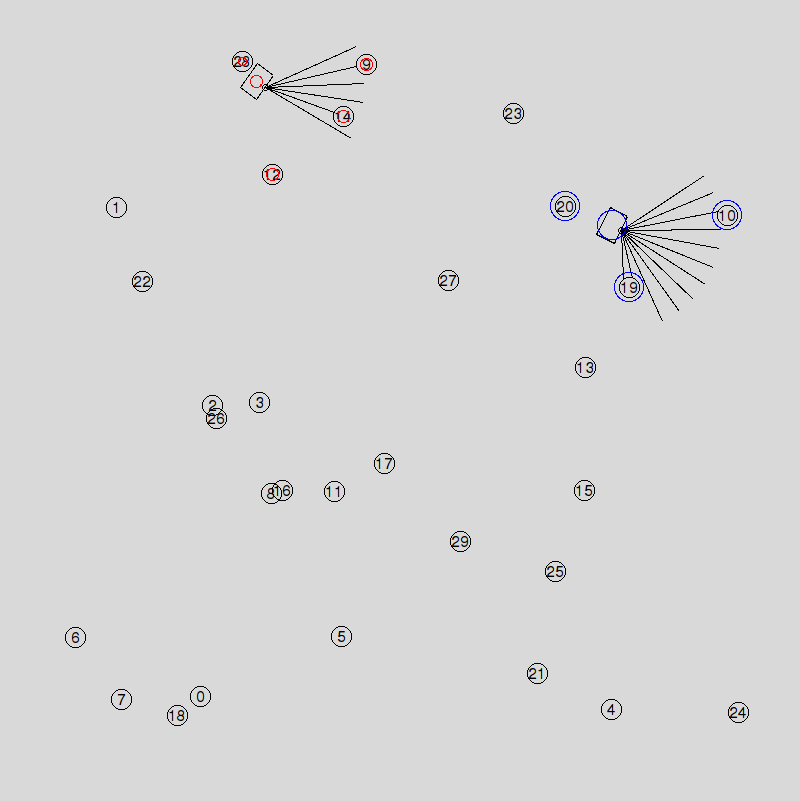
\includegraphics[width=\textwidth]{screenshot.png}
\caption{Simulation environment}
\end{figure}

The black circles represent unique landmarks.




We assume a simple linear system with gaussian transtion and sensor noise.  Covariance matrices express relationships between landmarks and robot positions and between landmarks themselves.  

A diagram of the system is shown below:

\begin{figure}[h!]
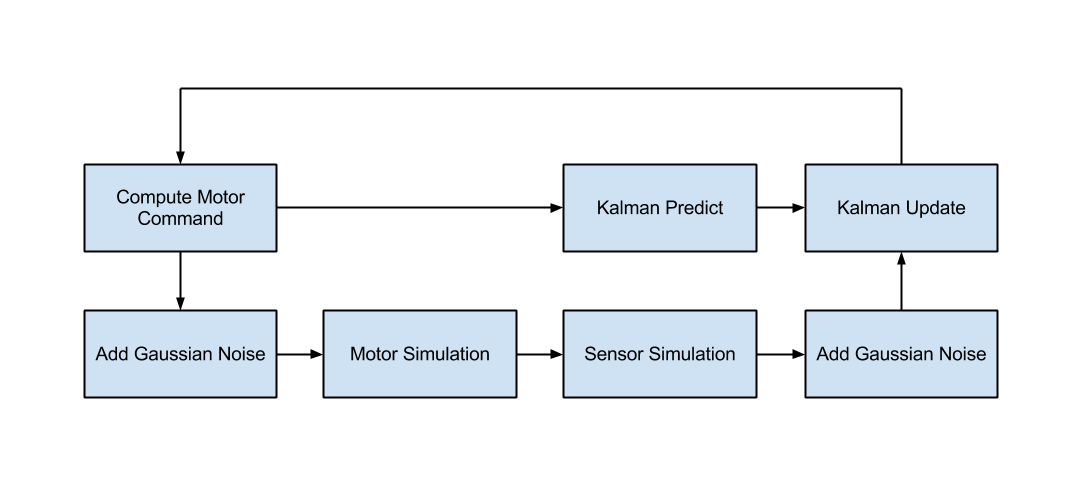
\includegraphics[width=\textwidth]{systemdiagram.png}
\caption{The flow of the program. Gaussian noise is added at the interfaces of the simulator to an uncertain environment.}
\end{figure}

Kalman Predict

Sense

Kalman Update




An example of our transition mode, $x' = x + Gu$:


$$
\begin{bmatrix}
    4 \\
    5 \\
    \pi \\
    l_{1x} \\
    l_{1y} \\
\end{bmatrix}
=
\begin{bmatrix}
    3 \\
    4 \\
    \pi  \\
    l_{1x} \\
    l_{1y} \\
\end{bmatrix}
+
\begin{bmatrix}
    1 & 0 & 0  \\
    0 & 1 & 0  \\
    0 & 0 & 1  \\
    0 & 0 & 0  \\
    0 & 0 & 0  \\
\end{bmatrix}
\begin{bmatrix}
    1 \\
    1 \\
    0 \\
\end{bmatrix}
$$

An example of our measurement model, $z = Hx$:

$$
\begin{bmatrix}
    mx_1 \\
    my_1 \\
    mx_2 \\
    my_2 \\
\end{bmatrix}
=
\begin{bmatrix}
    -1 & 0 & 0 & 1 & 0 & 0 & 0 & 0 & 0 \\
    0 & -1 & 0 & 0 & 1 & 0 & 0 & 0 & 0 \\
    -1 & 0 & 0 & 0 & 0 & 0 & 0 & 1 & 0 \\
    0 & -1 & 0 & 0 & 0 & 0 & 0 & 0 & 1 \\
\end{bmatrix}
\begin{bmatrix}
    x \\
    y \\
    \theta \\
    lx_1 \\
    ly_1 \\
    lx_4 \\
    ly_4 \\
    lx_2 \\
    ly_2 \\
\end{bmatrix}
$$



Some other stuff, yo what is this?




$$
u = 
\begin{bmatrix}
    \Delta x \\
    \Delta y \\
    \Delta \theta \\
\end{bmatrix}
$$

$$
z = 
\begin{bmatrix}
    x_1' \\
    y_1' \\
    x_2' \\
    y_2' \\
    x_3' \\
    y_3' \\
\end{bmatrix}
$$


$$
\vec{x}_i = \vec{x}_i - \langle x, y \rangle
$$







$$
\begin{bmatrix}
    x \\
    y \\
    \theta \\
\end{bmatrix}
\rightarrow
\begin{bmatrix}
    x \\
    y \\
    \theta \\
    l_{x_1} \\
    l_{y_1} \\
    l_{x_4} \\
    l_{y_4} \\
    l_{x_2} \\
    l_{y_2} \\
\end{bmatrix}
$$

$$
z = 
\begin{bmatrix}
    l_{1x} \\
    l_{1y} \\
    l_{2x} \\
    l_{2y} \\
\end{bmatrix}
$$

$$
P =
\begin{bmatrix}
    x_r & 0 & 0 & 0 & 0 & 0 & 0 & 0 \\
    0 & y_r & 0 & 0 & 0 & 0 & 0 & 0 \\
    0 & 0 & \theta & 0 & 0 & 0 & 0 & 0 \\
    1 & 0 & 0 & l_{1x} & 0 & 0 & 0 & 0 \\
    0 & 1 & 0 & 0 & l_{2x} & 0 & 0 & 0 \\
    0 & 0 & 0 & 0 & 0 & \ddots & 0 & 0 \\
    0 & 0 & 0 & 0 & 0 & 0 & l_{nx} & 0 \\
    0 & 0 & 0 & 0 & 0 & 0 & 0 & l_{ny} \\
\end{bmatrix}
$$








\subsection{Parameters}

\subsection{Motion Model}

\subsection{Sensor Model}

\subsection{Distributed SLAM}

To combine the results from multiple robots, we use another Kalman filter, with just a prediction step and no update.  Each robot's state vector is treated as a measurement and the covariance as the measurement noise.  The resulting estimates are fed back into each robot at each iteration.



\section{Results}

lol



\begin{thebibliography}{12}
    \bibitem{thrun2005}
        S. Thrun, W. Burgard, and D. Fox, \emph{Probabilistic Robotics}, MIT Press, 2005.

    \bibitem{thrun2003}
        S. Thrun and Y. Liu, ``Multi-Robot SLAM with Sparse Extended Information Filters'', \emph{Proceedings of the 11th International Symposium of Robotics Research (ISRR'03)}, 2003.

    \bibitem{cunningham2010}
        A. Cunningham, M. Paluri, and F. Dellaert, ``DDF-SAM: Fully Distributed SLAM using Constrained Factor Graphs'', \emph{International Conference on Intelligent Robots and Systems (IROS)}, 2010.

\end{thebibliography}









\end{document}
